%!TEX root = Slic3r-Manual.tex

\paragraph{Netfabb Studio} % (fold)
\label{par:netfabb_studio}
Netfabb produce a range of 3D modelling applications, including a free basic version\footnote{http://www.netfabb.com/basic.php}.  This version includes a mesh repair module which can help eliminate the various problems faced.  Up-to-date instructions can be found on the Netfabb wiki\footnote{http://wiki.netfabb.com/Part\_Repair}, the following is a quick overview of the steps involved.

\begin{figure}[H]
\centering
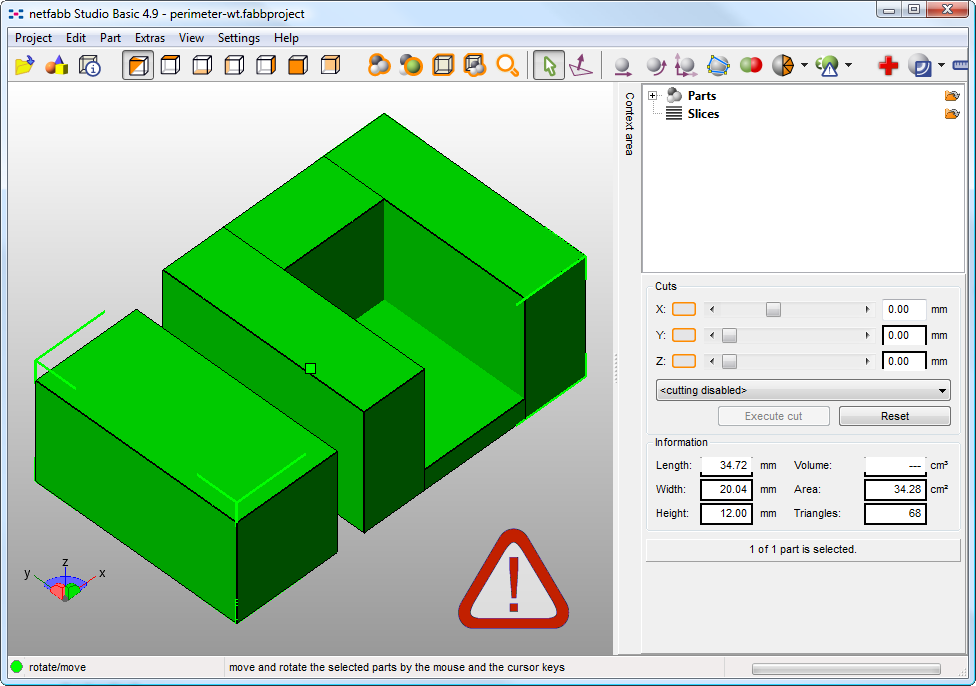
\includegraphics[keepaspectratio=true,width=0.75\textwidth]{working_with_models/netfabb_studio_part_repair.png}
\caption{Netfabb Studio: Part repair.}
\label{fig:netfabb_studio_part_repair}
\end{figure}

\begin{itemize}
	\item Start Netfabb Studio, and load the problem STL file, either via the \texttt{File} menu or by dragging and dropping it onto the workspace. If Netfabb detects a problem it will show a red warning sign in the bottom right-hand corner.
	\item To run the repair scripts, select the part and then either click the first aid icon in the toolbar (the red cross), or select from the context menu \texttt{Extras->Repair Part}.  This will open the part repair tab and show the status of the model.
	\item The \texttt{Actions} and the \texttt{Repair scripts} tabs offer several repair scripts which can be applied manually, however for the purposes of this overview selecting the \texttt{Automatic repair} script will fix most problems.
	\item The automatic repair button presents two options: Default and Simple.  Choosing Default will cover most cases. Select \texttt{execute} to run the scripts.
	\item Once the part is repaired the repairs must be applied by selecting \texttt{Apply repair}, choosing whether to override the existing part or not.
	\item The part may then be exported by selecting \texttt{Export part->As STL} from the context menu.
	\item If Netfabb still detects that the exported part will still contain errors then it will provide the option to apply further repairs before exporting.
	\begin{figure}[H]
	\centering
	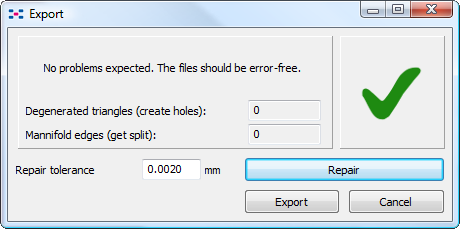
\includegraphics[keepaspectratio=true,width=0.75\textwidth]{working_with_models/netfabb_studio_export_part.png}
	\caption{Netfabb Studio: Part export.}
	\label{fig:netfabb_studio_export_part}
	\end{figure}
\end{itemize}
% paragraph netfabb_studio (end)

\paragraph{Netfabb Cloud Service} % (fold)
\label{par:netfabb_cloud_service}
Netfabb also hosts a web service where an STL file may be uploaded for it to be checked and repaired\footnote{http://cloud.netfabb.com/}.  

\begin{figure}[H]
\centering
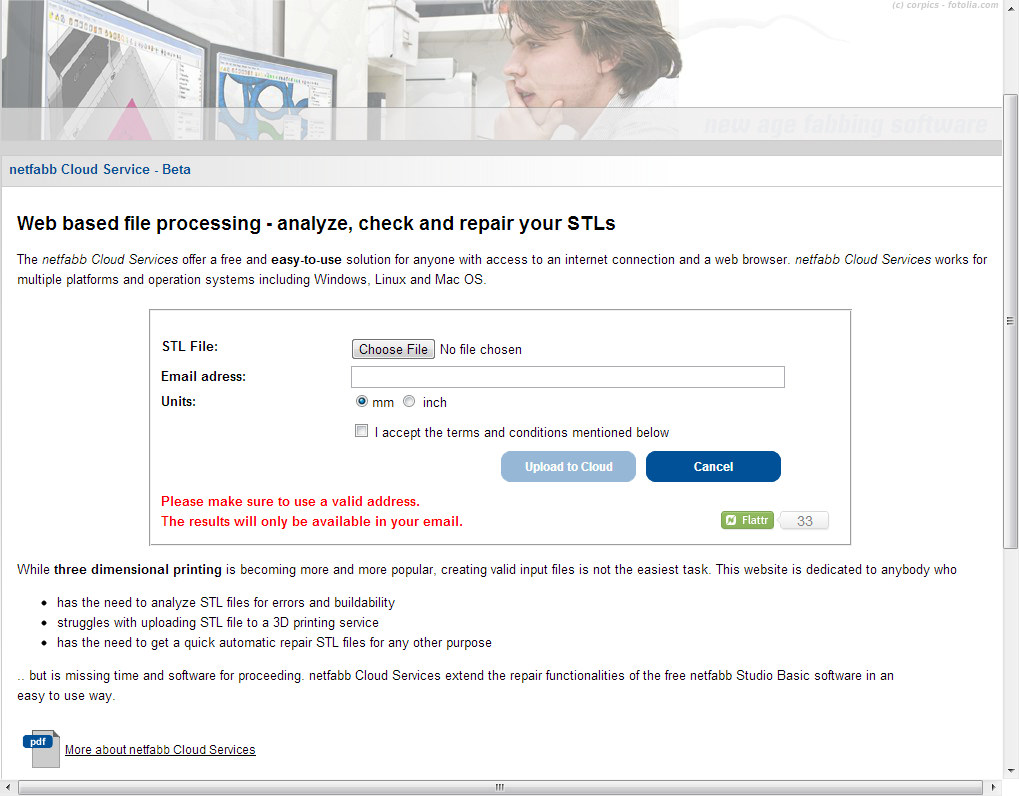
\includegraphics[keepaspectratio=true,width=0.75\textwidth]{working_with_models/netfabb_cloud_services.png}
\caption{Netfabb Cloud Services.}
\label{fig:netfabb_cloud_services}
\end{figure}

\begin{itemize}
	\item Navigate to http://cloud.netfabb.com
	\item Choose the STL file to upload using the button provided.
	\item An email address must be given to inform you when the service is finished.
	\item Choose whether metric or imperial measurements should be used.
	\item Read and accept the terms of service, and then click \texttt{Upload to Cloud}.
	\item Once the service has analysed and repaired the file an email is sent providing the download link to the repaired file.
\end{itemize}
